\documentclass[12pt]{article}
\usepackage{style}

\title{DL_Book 1_chapter}
\author{М.В. Ронкин, В.В. Зюзин }
\date{г. Екатеринбург, 2021}

\begin{document}
\begin{sloppypar}

 \newpage
\section{Глава 2. Введение в предмет Компьютерное зрение}

% \subsection{ }
\subsection{Предмет классической обработки изображений}
Предмет компьютерное зрение включает в себя изучение и применение фото изображений и их видео последовательностей для анализа и понимания реальных объектов или сцен, а также вопросы, относящиеся к реализации предложенных алгоритмов и их методологические проблемы \cite{Kettler2019computer}. 

Цифровое изображение можно описать как оцифрованное (дискретиазция и квантование) представление непрерывных аналоговых данных в пространственной области. Цифровое изображение состоит из прямоугольного массива пикселей ($x, y, u$). Каждый пискель является комбинацией местоположения $ ( x, y ) \in \mathcal{Z}^2 $ и значения интенсивности $u$.
% представляющего значения интенсивностей  нескольких, по сути, не зависимых цветовых каналов в точке $( x, y )$ (например цвета в формате RGB (red, green, blue). 
Здесь $\mathcal{Z}$ - множество всех целых чисел. Точки $(x, y)$  образуют регулярную сетку. Отметим, что формально  изображение $\mathcal{I}$ определено на прямоугольном множестве ${\Omega}$, которое называется носителем (carrier)  $\mathcal{I}$ и содержит узлы сетки: 
\begin{equation}
    \Omega = {(x, y): 1\leq x \geq W_{\text{кол}} \land 1\leq x \geq H_{\text{стр}} \subset {\cal Z}^2},
\end{equation}
где $W_{\text{кол}}, H_{\text{стр}}$ узлы сетки по горизонтали и  вертикали с равномерным шагом; $|\Omega|  = W_{\text{кол}} \cdot H_{\text{стр}}$ - мощность носителя \cite{Kettler2019computer}. 

Если изображение цветное, то изображение может представлять собой набор нескольких значений $u$, соответствующих нескольким цветовым каналам. Для любого оцифрованного изображения можно ввести его размер $W \times H\times C$, где $W,H$ - это ширина и высота изображения, $C$ - число каналов. 

Отметим, что как правило значения $x,y,u$ - дискретные. 
Причем часто $u$ выбираются в диапазоне $[0,255]$ - то есть в 8-ми битном диапазоне, а шаг изменений пространственных координат по x и y равномерный. 
Таким образом можно сказать, что оцифрованное изображение, как правило, имеете 8-битное квантование и дискретизацию с равномерным шагом $\Delta x = \Delta y = x_2-x_1$.  Если число каналов $C=1$ - то говорят об \textbf{одно-тоновых (монохромных) изображения}, часто принято визуализировать такие изображения в оттенках серого, однако на самом деле оттенки будут отражать значения яркости $u$ безотносительно какого бы ни было цвета. 
Также в ряде случаев мы будем иметь дело с бинарными изображениям. \textbf{Бинарные изображения} -  это изображения для которых $C=1, \ u= \{1,0\}$, такие изображения принято визуализировать с использованием только двух цветов: черного и белого \cite{Kettler2019computer}. 

Таким образом, каждое оцифрованное изображение может быть представлено в виде матрицы или нескольких матриц, объединенных в так называемый тензор (в упрощенном смысле этого слова). Отметим, что если изображение описывается одной матрицей, то это не цвета, а светимость (физическая интенсивность) или яркость (воспринимая интенсивность). Для описания цветных изображений основными способами описания являются формат RGB (red, green, blue) и HSI (hue, saturation, lightness (intensity) - тон, насыщенность, светлота), а также некоторые другие. Иллюстрация представления цвета $q$ в форматах RGB и HSI приведена на рисунке \ref{ch2:fig:rgb_hsi}\cite{Kettler2019computer}.

    \begin{figure}[h]
    	\begin{center}
    		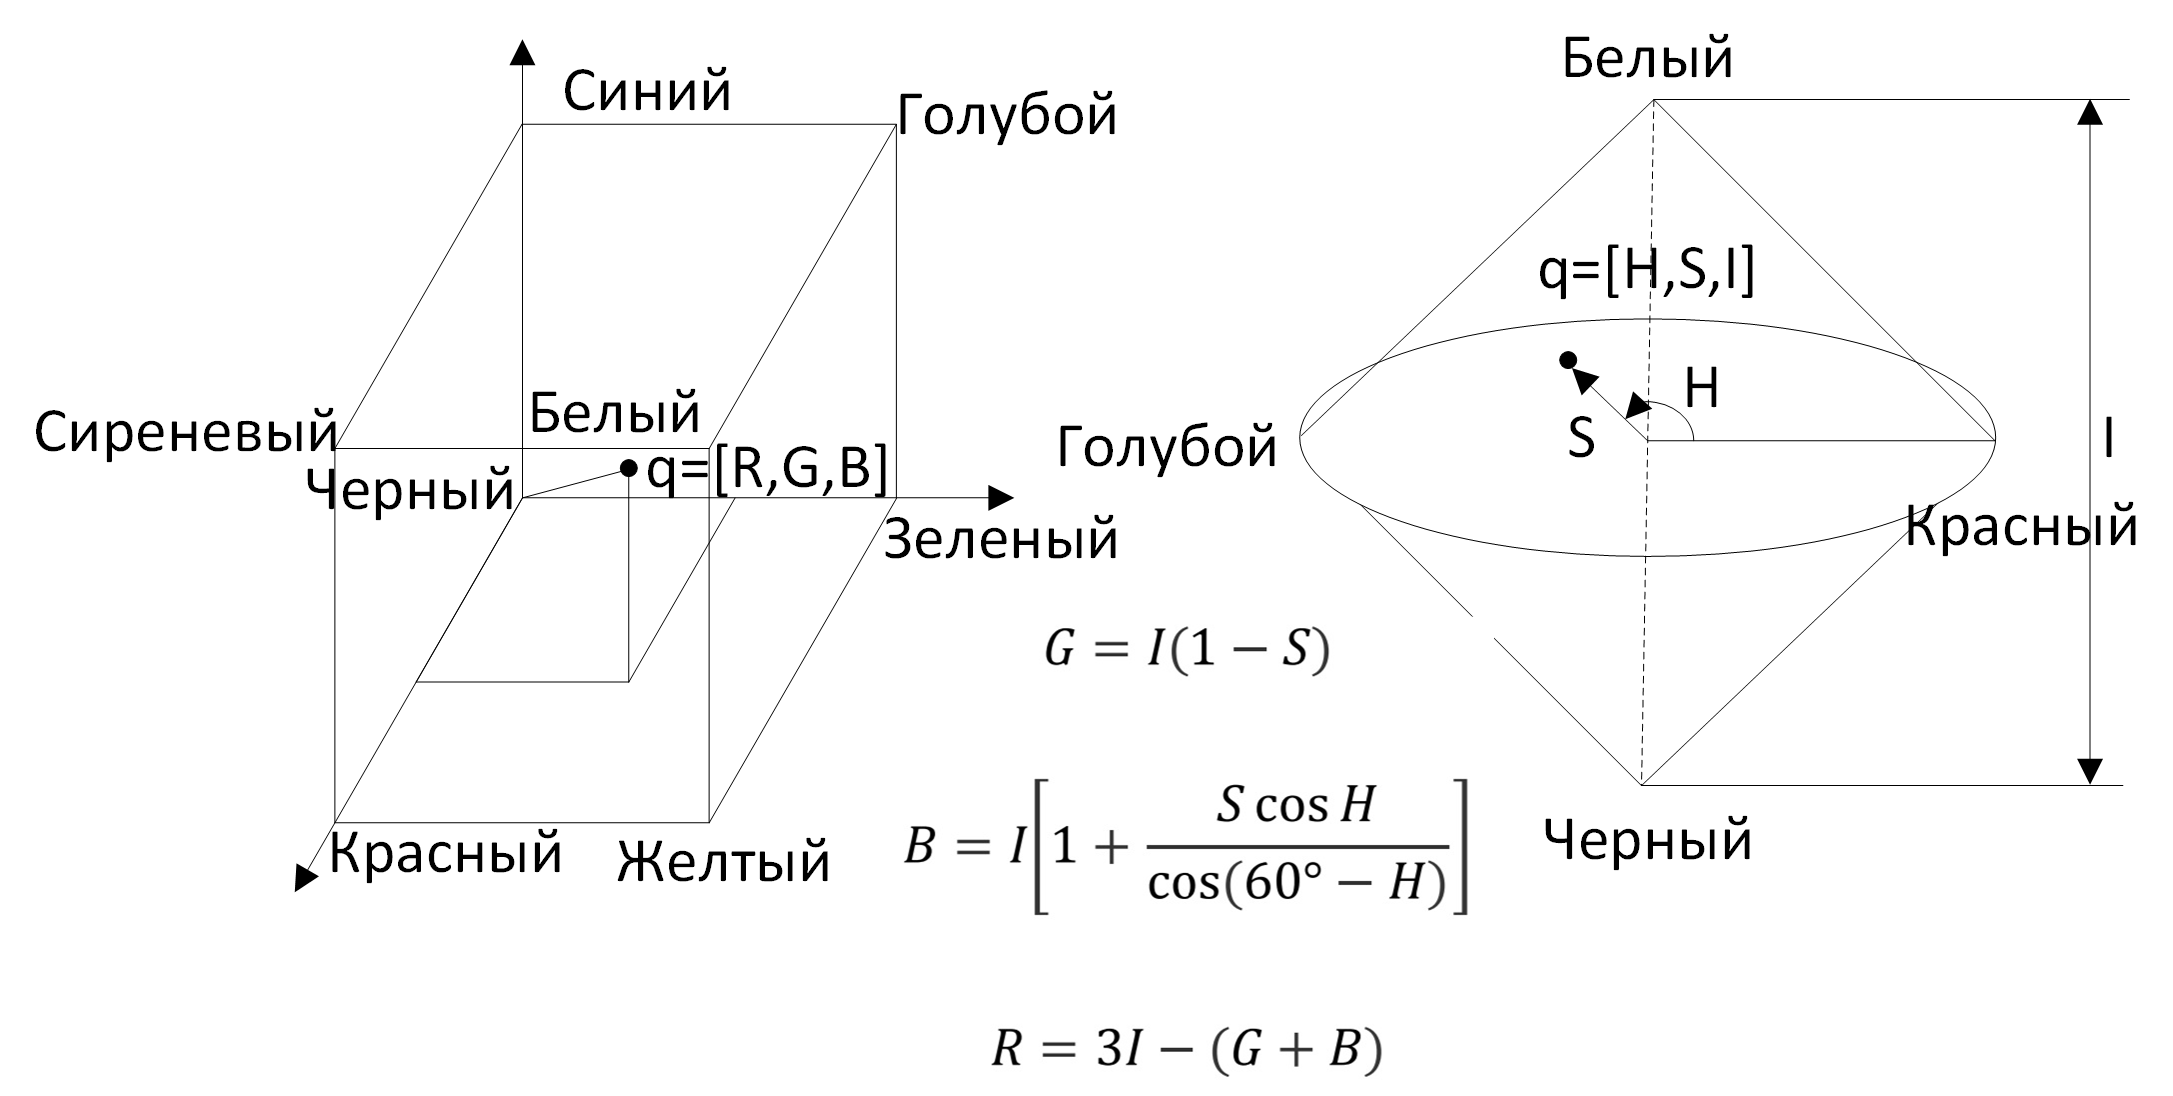
\includegraphics[width=0.99\linewidth]{./figuresch2/RGB_HSI.png}
    		\caption{Иллюстрация представления цвета $q$ в форматах RGB и HSI}		
    		\label{ch2:fig:rgb_hsi}
    	\end{center}
    \end{figure}

Для изображения можно ввести такие характеристики, как яркость, контрастность, гистограмма яркости и другие \cite{Kettler2019computer}.
\begin{itemize}
    
    \item \textbf{Средняя яркость изображения} может быть вычислена как 
        \begin{equation}
            \mu_I = \dfrac{1}{|\Omega|}\sum_{x=0}^{W-1}\sum_{y=0}^{H-1}I(x,y),
        \end{equation}
        где $\mu_I$ - средняя яркость; $|\Omega| = W\cdot H$.
   
    \item \textbf{Контрастность} - средняя разность значений яркости каждого пикселя и соседних к нему
        \begin{equation}
           \nu = 
           \dfrac{1}{|\Omega|}\sum_{x=0}^{W-1}\sum_{y=0}^{H-1}|I(x,y)-\mu_w(x,y)|,
        \end{equation}
        где $\nu$ - контрастность; $\mu_w(x,y)$ - среднее по окну пискселей вокруг пикселя с координатами.
    
    \item \textbf{Гистограмма яркости} может быть выражена как подсчет числа раз, когда встречается то или иное значение яркости канала $u$:
        \begin{equation}
            H(u) = |\{(x,y)\in \Omega: I(x,y) = u\}|, \quad
            h(u) =\dfrac{H(c)}{|\Omega|}, \quad
            CDF(u) = \sum_{v=0}^{u-1}h(u)
        \end{equation}
        где $H(u)$ - абсолютная гистограмма; $h(u)$ - относительная гистограмма; $CDF(u)$ - кумулятивная функция гистограммы. \newline
        Гистограмма определяет распределение яркости по каждому оттенку цветового канала (число раз сколько встречается тот или иной оттенок $u$). Кумулятивная функция гистограммы показывает сколько раз встречаются все значения яркости вплоть до выбранного. Иллюстрации гистограммы одного и того же изображения, имеющего различную яркость приведены на рисунке \cite{ch2:fig:histogram}.
 
    \item \textbf{Частотное представление изображения} (спектральное представление). Частотным является представление изображение в виде его разложение по двух-мерному ортогональному базису, например Фурье базису. То есть, в наиболее простом случае, частотное представление это двух-мерное преобразование Фурье от изображения. Результатом такого преобразования в общем случае является набор двух-мерных комплексных величин $\mathbf{I}(k,j)$,
    где $k,j$ - это т.н. пространственные частоты. Д\textbf{вухмерное прямое дискретное преобразование Фурье} может быть записано как
        \begin{equation}
           \mathbf{I}(k,j) = \dfrac{1}{|\Omega|}\sum_{x=0}^{W-1}\sum_{y=0}^{H-1}I(x,y)\exp\left(-i2\pi\left(\dfrac{xk}{W}+\dfrac{yj}{H}\right)\right),
        \end{equation}
    где $i = \sqrt{-1}$. \newline
    Преобразование Фурье показывает, что изображение может быть разложено набор гармонических базисных функций вида $\exp(-i2\pi(\dfrac{xk}{W}+\dfrac{yj}{H}))$. Как правило рассматривается только амплитудная часть спектра $|\mathbf{I}(k,j)|$. Для амплитудного спектра можно сделать следующие выводы. Наличие интенсивности изображения для функций с наиболее низкой (около-нулевой) частотой соответствует однородным частям массива. Наличие интенсивности для низких частот будет соответствовать медленно меняющимся частям изображения (например, размытие). Наличие интенсивности на высоких частотах, напротив, будет соответствовать резко-изменяющимся частям массива, например, контрастным границам. Примеры иллюстраций амплитудных спектров для некоторых изображений приведены на рисунке \ref{ch2:fig:spectrum}. Следует отметить, что на практике преобразование Фурье как правило реализуется при помощи  т.н. \textbf{алгоритма Быстрого преобразования Фурье (БПФ, Fast Fourier Transform, FFT)}.
\end{itemize}

    \begin{figure}[!h]
    	\begin{center}
    		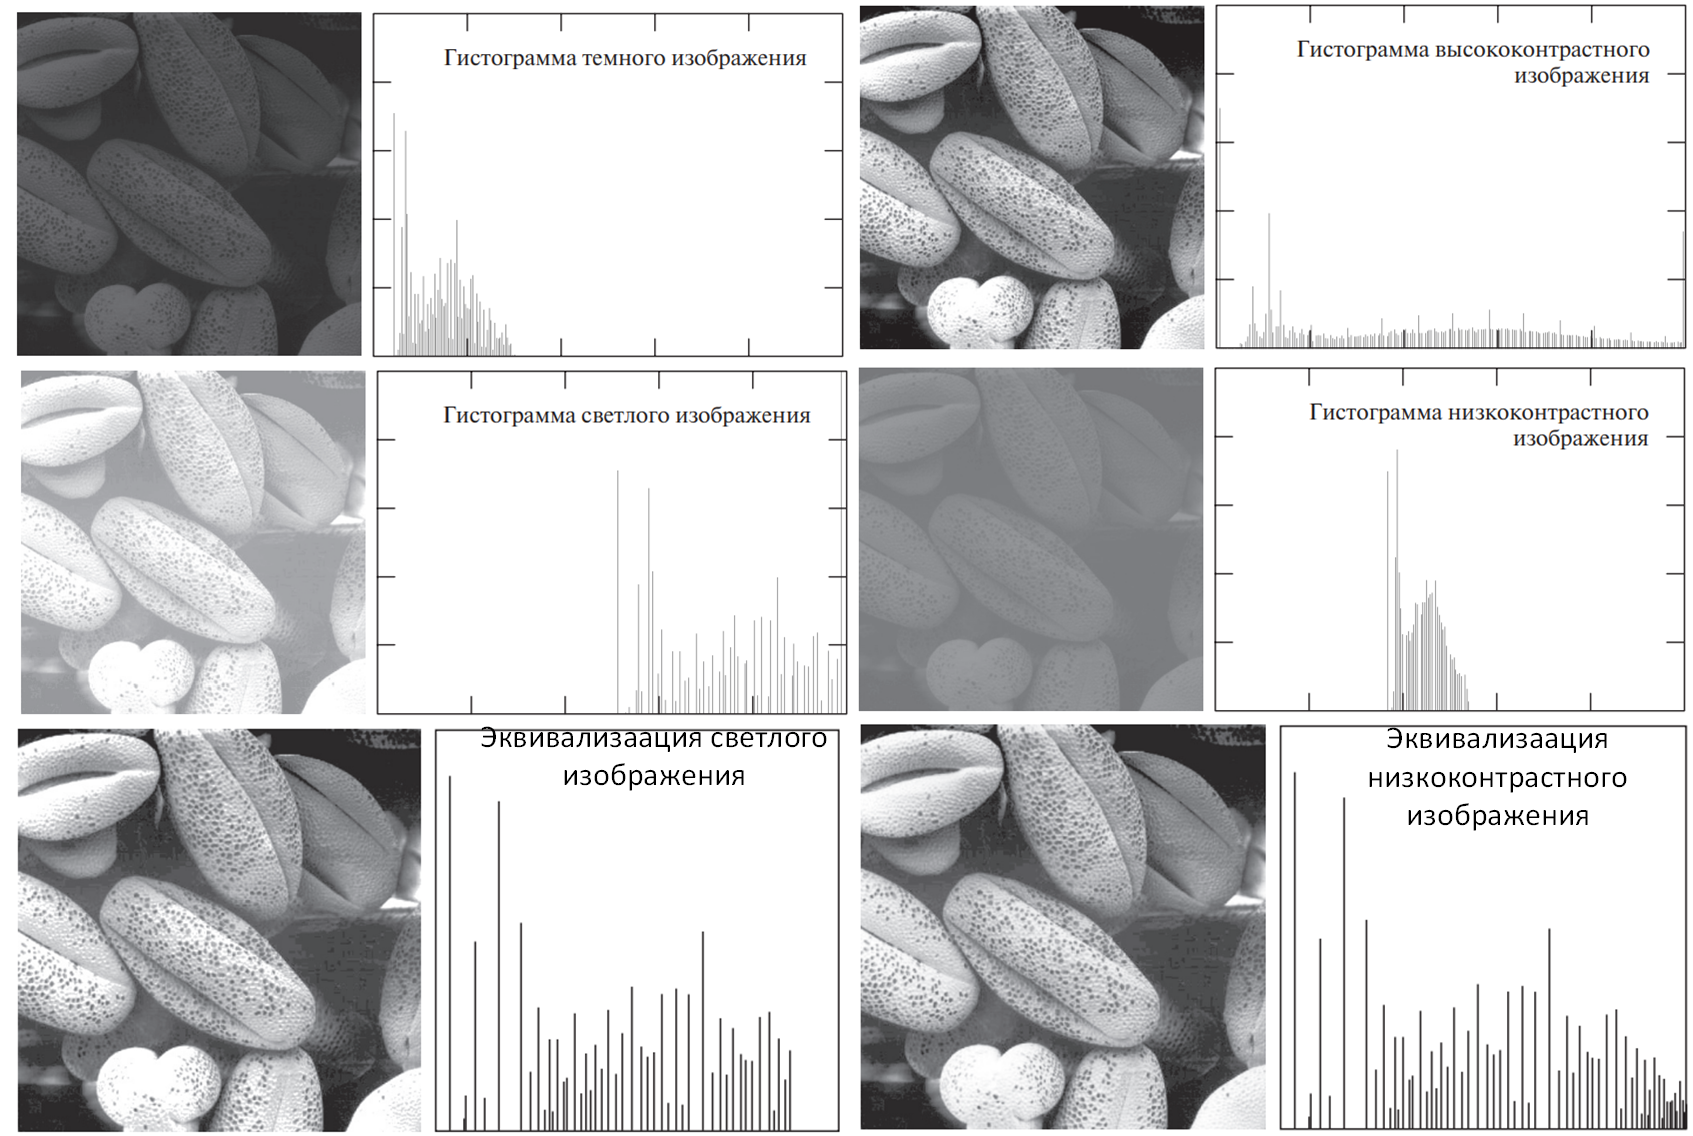
\includegraphics[width=0.69\linewidth]{./figuresch2/Histogramm.png}
    		\caption{Иллюстрации гистограммы яркости изображений}		
    		\label{ch2:fig:histogram}
    	\end{center}
    \end{figure}

    \begin{figure}[!h]
    	\begin{center}
    		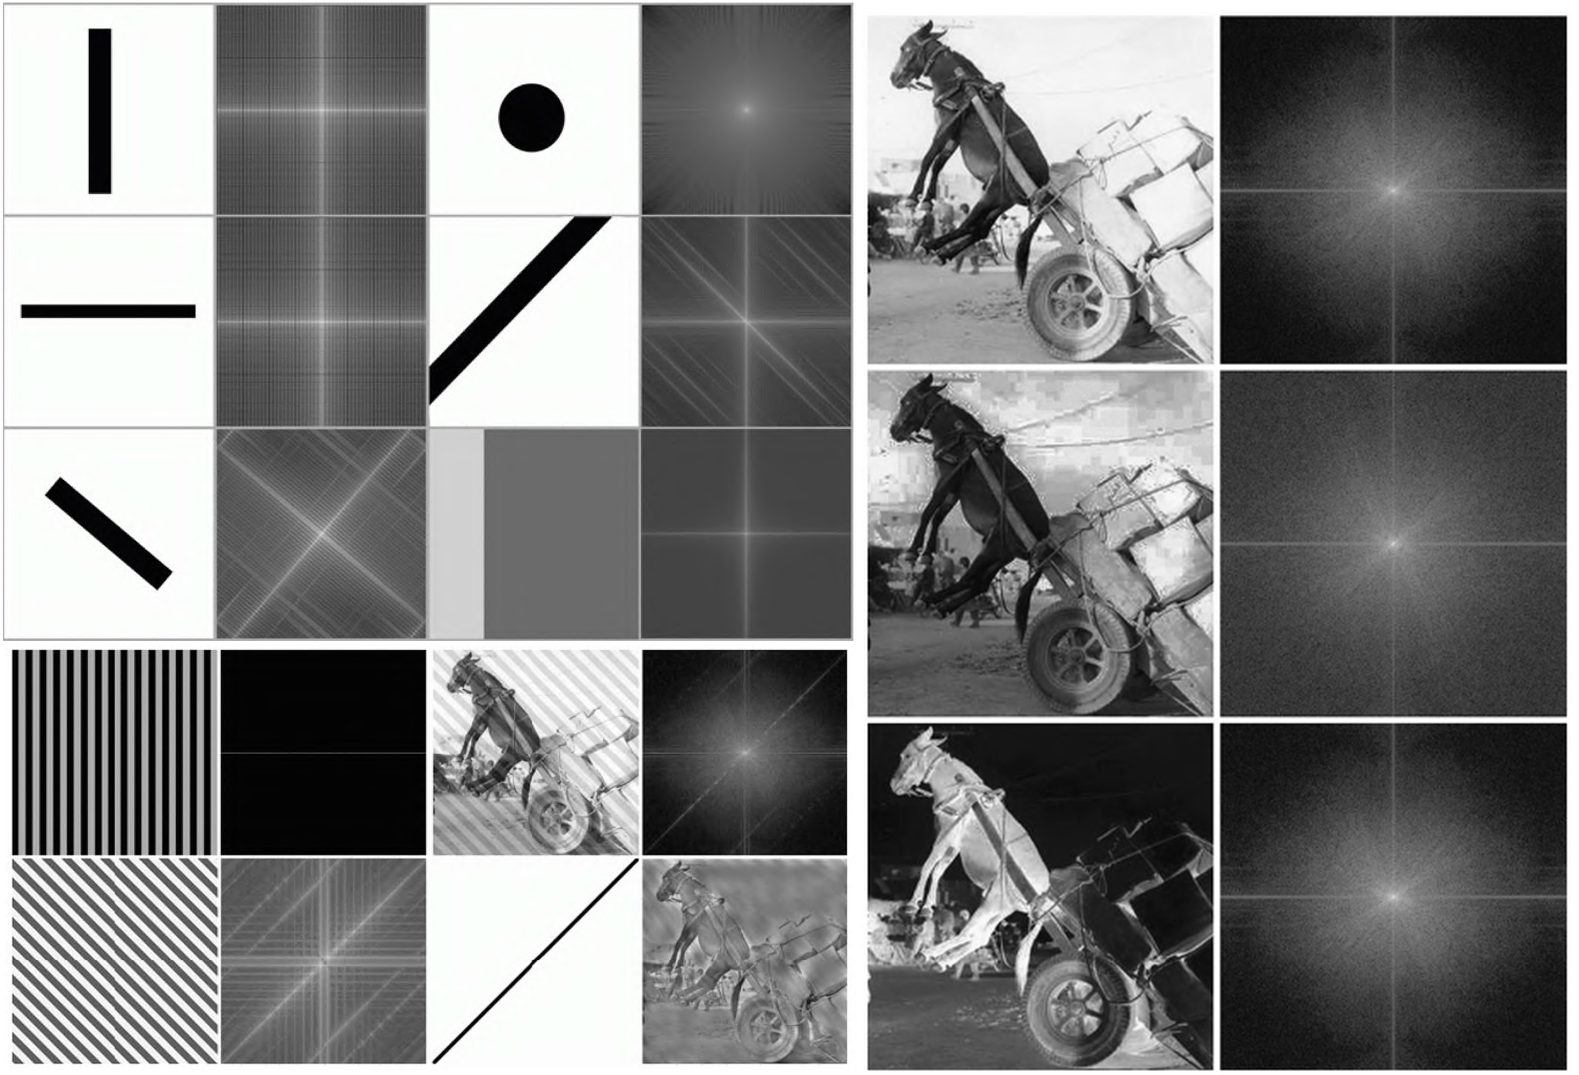
\includegraphics[width=0.99\linewidth]{./figuresch2/spectrum.png}
    		\caption{Иллюстрации амплитудных спектров некоторых изображений}		
    		\label{ch2:fig:spectrum}
    	\end{center}
    \end{figure}
Отметим, что дискретное представление изображений приводит к ряду ограничений.  Наиболее существенное из которых - частотное ограничение. Данное ограничение связано с условиями Теоремы Котельникова. 

\textbf{Теорама Котельникова (теорема Котельникова-Шенона-Найквиста) для цифровых изображений}  теорема сводится к тому, что максимальная пространственная частота в изображении не может быть выше чем $1/2\Delta x$. Таким образом спектр цифрового изображения ограничен. Это можно представить как ограничение резкости оцифрованного изображения. Так, для изображений низкого разрешения нельзя получить высокое качество выделения границ, особенно для небольших объектов.  Если в спектре изображения должны появится высокие частот, то это приводит к т.н. артефактам наложения - то есть эффектам точечного искажения. Такой эффект называется\textbf{ эффект алиасигна}.

 \subsection{Операции классической обработки изображений}
Предмет классической обработки изображений изображений - это достаточно большой курс и широко развитая область знаний. В данной книге эти вопросы не будут рассмотрены. Однако, интересующийся читатель может найти информацию, например, в таких книгах, как
\cite{Gonsales2019Digital, Jane2011Digital, solomon2011fundamentals} и многих других.

Операции классической обработки изображений включают следующие типы \cite{Gonsales2019Digital}.
\begin{itemize}
    \item \textbf{Градационные преобразования} (попиксильные преобразования яркости) например,:
    усиление контраста, инверсия (получение негатива), степенная, кусочно-линейная, логорифмическая или другая нелинейная коррекция яркости.
   \item \textbf{Гистограммные преобразования},  например,:   локальное или глобальное выравнивание гистограммы (эквивализация), приведение гистограммы к заданному виду или ее масштабирование.
   \item \textbf{Пространственная фильтрация изображений}. Данный тип операций основан на т.н. операции пространственной свертки, речь о которой пойдет ниже. 
   \item \textbf{Нелинейная фильтрация изображений}. Данный тип операций основан, например, на использовании порядковых статистик (медианный фильтра), операциях расчета градиентна от изображения или на использовании нечетких множеств.
   \item \textbf{Передискретизация изображений}. Данный тип операциях прореживания и/или интерполяции  значений пикселей с целью изменения общего размера изображения.
   \newline 
\end{itemize} 

\textbf{Операция пространственной свертки (двухмерная свертка, convolution)} является широким понятием, которое возникает в различных приложениях статистической обработки данных. По существу, операция сводится к оценки "схожести" двух функций, скажем, $I(x,y)$ и $G(-x,-y)$, одна из которых смещается относительно другой как по оси $x$, так и по оси $y$. В данном определении операция свертки соответствует взаимокорреляционной функции между $I(x,y)$ и $G(x,y)$. Свертка может быть использована, например,
\begin{itemize}
\item для поиска в изображении $I(x,y)$ некоторых шаблонов (патернов, образов, patterns) похожих на шаблоны, заданные в $G(x,y)$;
\item для проведение пространственной фильтрации, например, высокочастотная фильтрация оставит только наиболее резкие участки изображения, такие, как границы объектов. 
\end{itemize} 
Математически операция свертки может быть описана как
\begin{equation}
    r(x,y) = (G\ast I)(x,y) = \sum_{h=0}^{H_G-1}\sum_{w=0}^{W_G-1}G(h,w)I(x+h,y+w), 
    \label{ch2:eqn:conv} 
\end{equation}
где:
\begin{itemize}
\itemsep 0em 
    \item $G(h,w)$ - значение ядра свертки с для пикселя с координатами $(h,w)$ ($G$ имеет размерность $H_G \times H_G)$;
    \item $I(x,y$ - значение входного двухмерного массива с координатами $(x,y)$ ($I$ имеет размерность $H_I \times W_I$);
    \item $r(x,y)$ - значение результата свертки с координатами  $(x,y)$ ($r$ имеет размерность $H_I-H_G+1 \times W_I - W_H +1$);
    \item $\ast$ - операция свертки.
\end{itemize}
На практике операция пространственной свертки как правило проводится между изображением и т.н. окном (window), которое также может быть названо ядро свертки (kernel). Тогда операция
свертки может быть представлена так, как это показано на рисунках \ref{ch2:fig:2d_conv_stride_1_v2} и \ref{ch2:fig:2d_conv_stride_1} в двух разных формах. 
\begin{figure}[!h]
	\begin{center}
		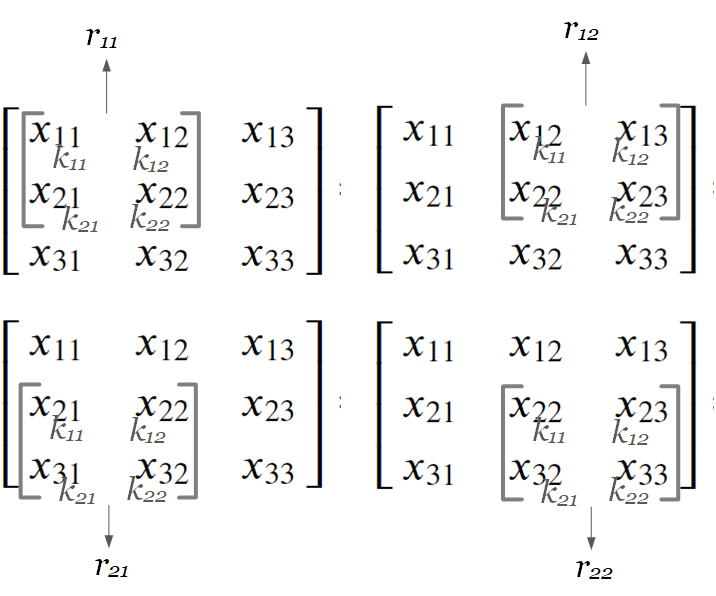
\includegraphics[width=0.7\linewidth]{./figuresch1/2d_conv_stride_1_v2.png}
		\caption{Иллюстрация двухмерной свертки $2 \times 2$}		
		\label{ch2:fig:2d_conv_stride_1_v2}
% 	\end{center}
% \end{figure}

% \begin{figure}
% 	\begin{center}
		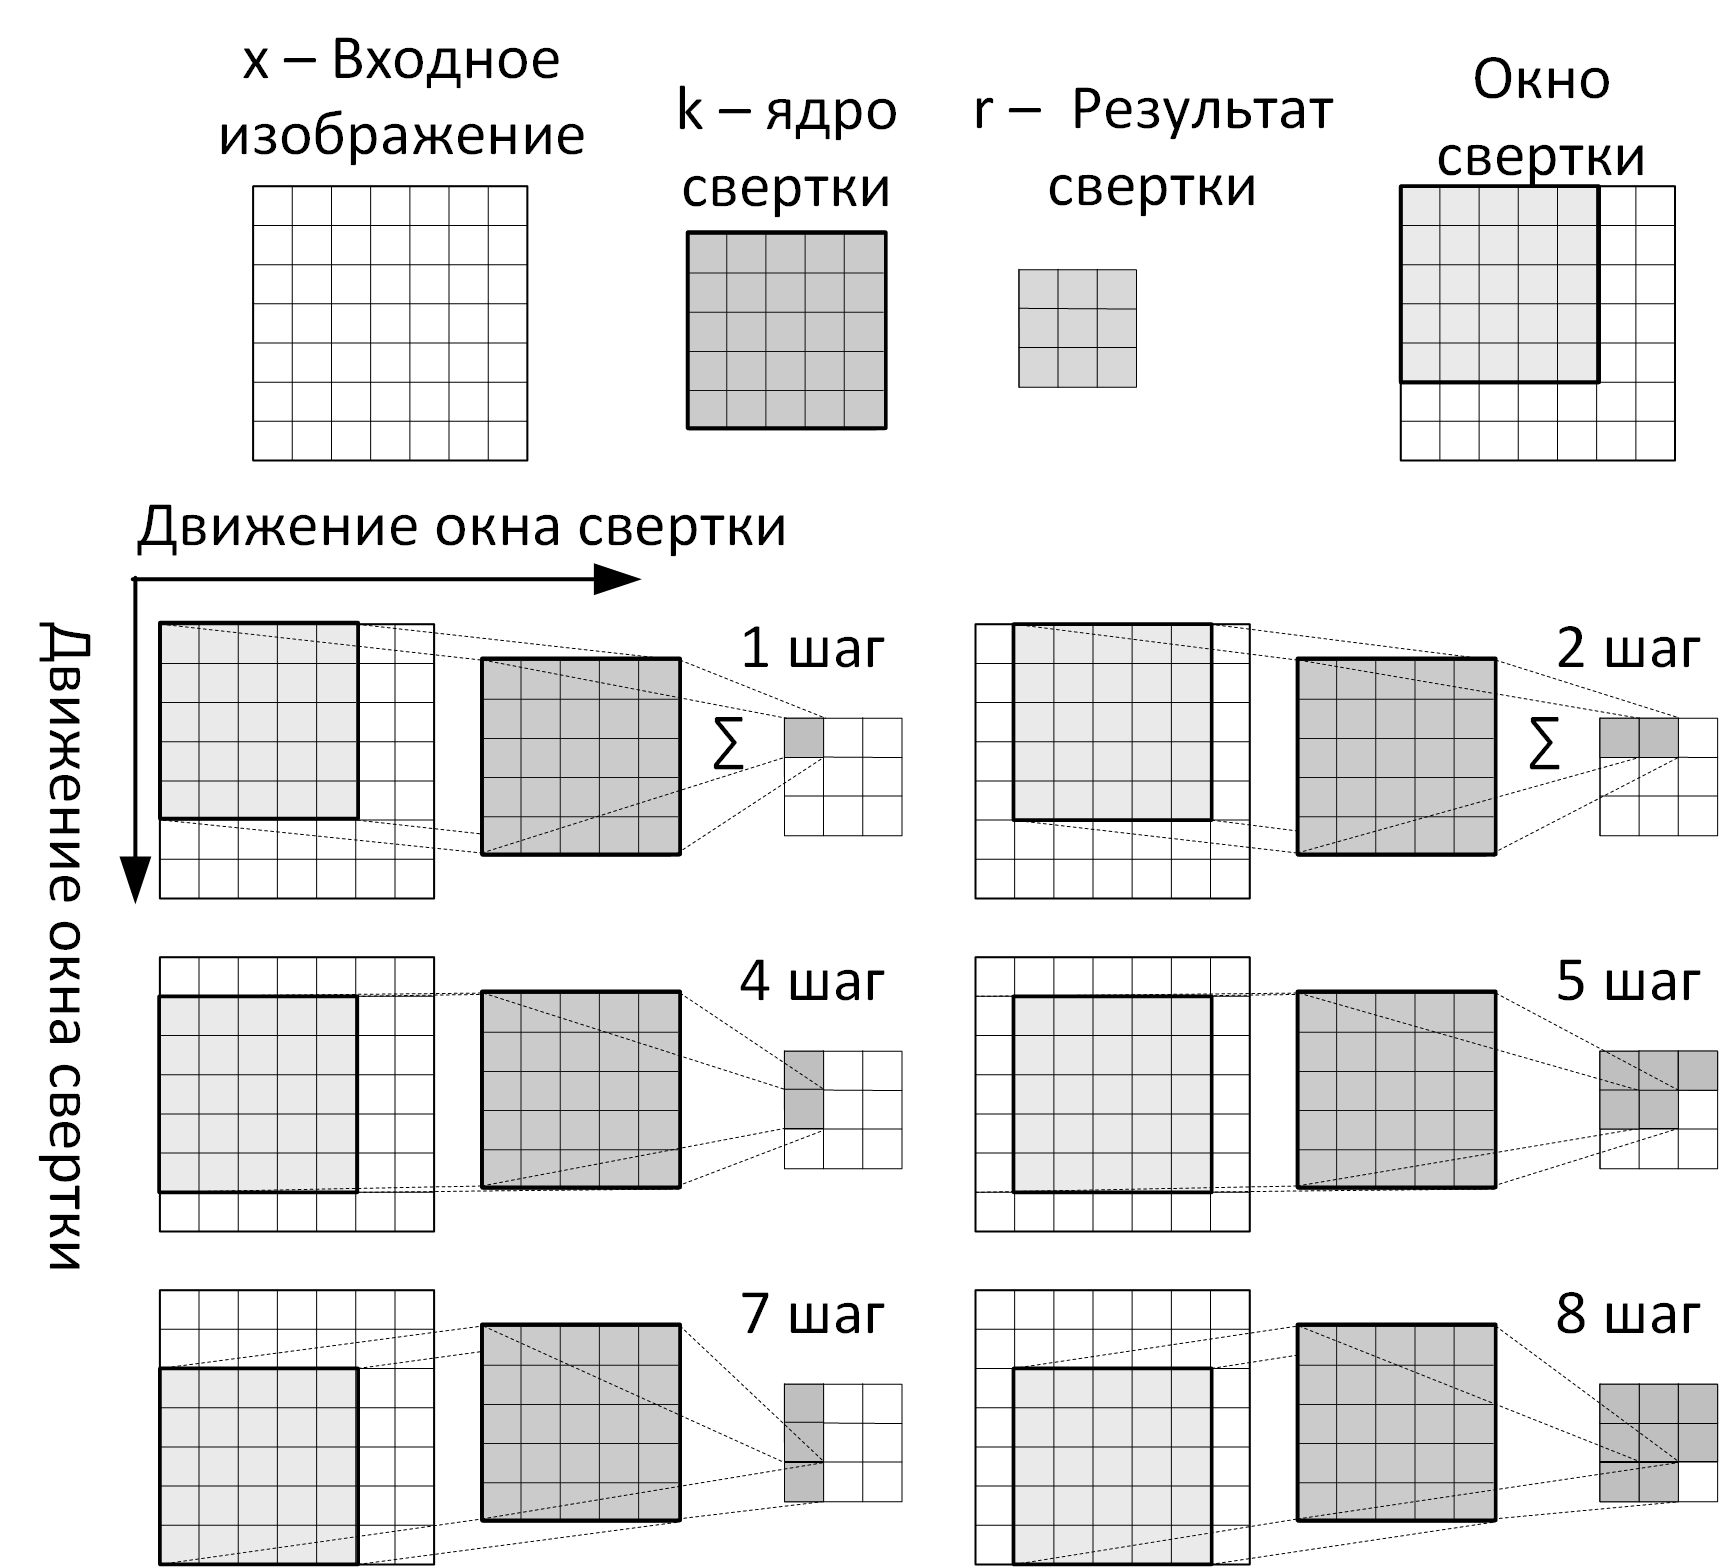
\includegraphics[width=0.76\linewidth]{./figuresch1/2d_conv_stride_1_v3.png}
		\caption{Иллюстрация двухмерной свертки $5 \times 5$}		
		\label{ch2:fig:2d_conv_stride_1}
	\end{center}
\end{figure}
Отметим, что здесь и далее предполагается, что направление движения окна фильтра слева на права и сверху вниз. Также отметим, что операция корреляции соответствует операции фильтрации с окном перевернутым на 180 градусов.

Как можно заметить из выражения (\ref{ch2:eqn:conv}) в общем случае операция свертки может привести к сокращению размеров изображения. Для того, чтобы этого не было перед сверткой изображение  может быть дополнено границей из нулей с шириной с каждого блока по горизонтали $H_G/2-1$; по вертикали $W_G/2-1$. Операция дополнения нулями называется \textbf{padding} или zero padding если быть более конкретным.

Часто, особенно в классической обработке изображений, для вычисления свертки вместо формулы (\ref{ch2:eqn:conv}) используют важное свойство свертки, которое может быть записано как
\begin{equation}
    r = (G\ast I) = {\mathrm{FFT}}^{-1}(\mathbf{I}\cdot\mathbf{G}),
    \label{ch2:eqn:conv} 
\end{equation}
где $\mathbf{I}$ и $\mathbf{G}$ - это Фурье-спектры изображения и ядра свертки, имеющие равный размер; ${\mathrm{FFT}}^{-1}$ - операция обратного преобразования Фурье.  Если операция выполняется между функциями разной размерности, то изображение меньшей размерности должно быть дополнено нулями с краев до равных значений со вторым изображением.
Также операция преобразования Фурье выполняется для изображений четной размерности.


https://arxiv.org/ftp/arxiv/papers/1910/1910.13796.pdf
Deep Learning vs. Traditional Computer Vision


%%%%%%%%%%%%%%%%%%%%%%%%%%
\newpage
\bibliography{bibl}

\end{sloppypar}
\end{document}
